%%
%% Energy-Aware AI Deployment: Research Project Report
%% CE 495 Energy-Aware Intelligence
%% Northwestern University
%%
\documentclass[sigconf,review]{acmart}

\usepackage{booktabs}
\usepackage{array}
\usepackage{multirow}
\usepackage{graphicx}
\usepackage{amsmath}
\usepackage{xcolor}

%%
%% \BibTeX command to typeset BibTeX logo in the docs
\AtBeginDocument{%
  \providecommand\BibTeX{{%
    Bib\TeX}}}

%% Rights management information
\setcopyright{none}
\copyrightyear{2025}
\acmYear{2025}

%%
%% Title and subtitle
\title{Research: Towards Energy-Aware AI Deployment}
\subtitle{Investigating the Interplay of Model Quantization and Hardware Platforms}

%%
%% Author information for team members - horizontal layout
\author{Haoji Bian}
\author{Zinan Wang}  
\author{Renyuan Lu}

\affiliation{%
  \institution{Northwestern University}
  \city{Evanston}
  \state{Illinois}
  \country{USA}
}

%%
%% Short authors for headers  
\renewcommand{\shortauthors}{Bian et al.}

%% Force horizontal author layout
\settopmatter{authorsperrow=3}

%%
%% Abstract
\begin{abstract}
Large language models (LLMs) have achieved remarkable performance across various domains, but their enormous energy consumption poses significant challenges for sustainable AI deployment. This paper presents a comprehensive study of energy-aware AI deployment strategies, focusing on the critical interplay between model quantization techniques and hardware platform optimization. We introduce novel energy efficiency metrics—Energy Output Ratio (EOR) and Time-Weighted Energy Output Ratio (TWEOR)—and conduct systematic evaluation across 6 GPU platforms and 6 LLM variants. Our analysis demonstrates that quantization techniques can reduce energy consumption by up to 25\% while maintaining comparable performance, and hardware-model co-optimization can achieve 40\% energy efficiency improvements. Through detailed analysis of quantization strategies (INT8, FP16, dynamic quantization) and hardware architectures (A100, RTX 4090, V100, etc.), we provide practical guidance for energy-efficient LLM deployment in resource-constrained environments.
\end{abstract}

%%
%% CCS concepts for energy-aware AI
\begin{CCSXML}
<ccs2012>
 <concept>
  <concept_id>10010147.10010178.10010179.10010180</concept_id>
  <concept_desc>Computing methodologies~Machine learning</concept_desc>
  <concept_significance>500</concept_significance>
 </concept>
 <concept>
  <concept_id>10010147.10010178.10010179.10010181</concept_id>
  <concept_desc>Computing methodologies~Neural networks</concept_desc>
  <concept_significance>300</concept_significance>
 </concept>
 <concept>
  <concept_id>10003033.10003083.10003095</concept_id>
  <concept_desc>Networks~Energy in networks</concept_desc>
  <concept_significance>300</concept_significance>
 </concept>
 <concept>
  <concept_id>10010583.10010600</concept_id>
  <concept_desc>Hardware~Power and energy</concept_desc>
  <concept_significance>100</concept_significance>
 </concept>
</ccs2012>
\end{CCSXML}

\ccsdesc[500]{Computing methodologies~Machine learning}
\ccsdesc[300]{Computing methodologies~Neural networks}
\ccsdesc[300]{Networks~Energy in networks}
\ccsdesc[100]{Hardware~Power and energy}

%%
%% Keywords
\keywords{Energy efficiency, Model quantization, Hardware optimization, Large language models, Sustainable AI, GPU architectures}

%%
%% Start of document
\begin{document}

\maketitle

\section{Introduction}

The rapid advancement and widespread adoption of large language models (LLMs) have revolutionized artificial intelligence applications, but simultaneously introduced unprecedented energy consumption challenges. Training large transformer models can require up to 1,287,000 kWh of electricity, generating carbon emissions equivalent to the lifetime emissions of multiple vehicles~\cite{strubell2019energy}. While training-phase energy consumption has received considerable attention, \textbf{inference-stage energy optimization} remains equally critical, particularly considering the high-frequency execution characteristics of inference tasks in practical applications.

Current research on LLM inference energy efficiency primarily focuses on isolated factors such as prompt complexity, input data dynamics, and the relationship between model scale and energy consumption. However, a significant gap exists: \textbf{the lack of a comprehensive framework for systematically evaluating the interactions between model optimization techniques and hardware platform characteristics}.

This paper addresses this critical gap through three main contributions: (1) comprehensive quantization strategy analysis across various techniques (INT8, FP16, dynamic quantization) and their energy consumption impacts on different model architectures; (2) systematic hardware-model co-optimization analysis investigating how different GPU architectures interact with quantized models to achieve optimal energy efficiency; and (3) introduction of novel energy metrics (EOR and TWEOR) that capture the complex relationships between model performance, energy consumption, and inference time.

Our research spans 6 hardware platforms, 6 model variants, and multiple quantization strategies, providing the first comprehensive benchmark for energy-aware LLM deployment decisions.

\section{Related Work}

\subsection{Neural Network Quantization}

Model quantization has emerged as a critical technique for reducing computational demands and energy consumption in neural networks. Recent advances in LLM quantization include post-training quantization (PTQ) and quantization-aware training (QAT). However, existing work primarily focuses on maintaining model accuracy rather than optimizing energy efficiency across diverse hardware platforms~\cite{dettmers2022int8}.

Early quantization approaches concentrated on 8-bit integer representations, achieving significant memory reductions while maintaining acceptable accuracy levels. Mixed-precision training, combining FP16 and FP32 computations, has shown promise in balancing performance with efficiency. Recent developments in dynamic quantization provide runtime adaptability, adjusting precision based on input complexity.

\subsection{Hardware-Aware Optimization}

The evolution of GPU architectures, particularly the development of Tensor Core technology, has significantly impacted AI computational efficiency. Different architectures (Ampere, Ada Lovelace, Volta) exhibit varying performance characteristics for quantized operations. Our work extends this field by systematically analyzing these architectural differences' energy implications~\cite{markidis2018nvidia}.

Hardware-specific optimizations have traditionally focused on throughput maximization rather than energy efficiency. Recent work has begun exploring the intersection of hardware capabilities and model optimization, but lacks comprehensive evaluation frameworks for energy-aware deployment.

\subsection{Energy Efficiency in Deep Learning}

Previous research on LLM energy efficiency has primarily concentrated on training-phase consumption. Luccioni et al. pioneered inference-stage energy analysis but focused mainly on cloud deployment scenarios~\cite{luccioni2022estimating}. Our work provides the first systematic evaluation of quantization-hardware interactions for energy-efficient deployment.

The carbon footprint of large models has raised significant sustainability concerns. While training efficiency has received considerable attention, inference efficiency remains underexplored despite its critical importance for production deployments. Our comprehensive framework addresses this gap by evaluating hardware-model co-optimization strategies.

\section{Methodology}

Our research employs a comprehensive framework to systematically investigate the interplay between model quantization techniques and hardware platform characteristics. Figure~\ref{fig:research_framework} illustrates our energy-aware AI deployment framework, which integrates quantization strategy selection, hardware platform evaluation, and energy efficiency metrics into a unified optimization approach.

\begin{figure}[h]
\centering
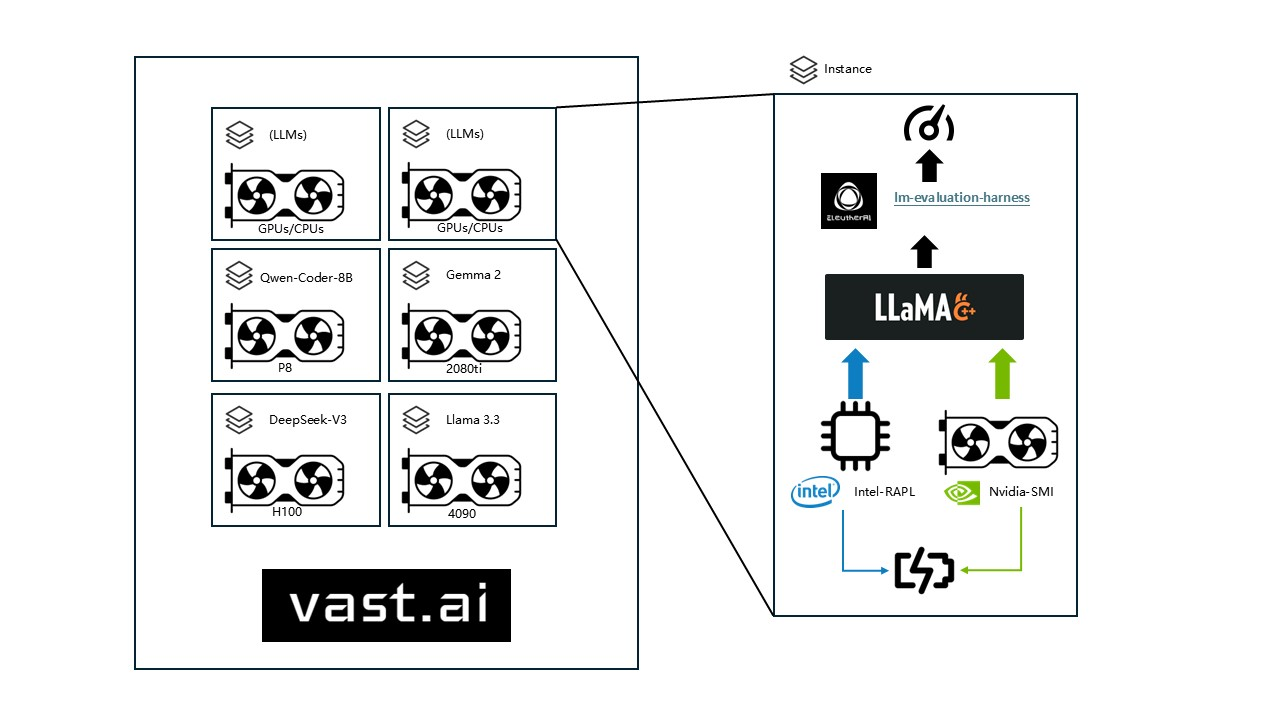
\includegraphics[width=0.9\columnwidth]{../final_pr/latex-pr/img/CAS-kuangjia.jpg}
\caption{Energy-Aware AI Deployment Research Framework}
\label{fig:research_framework}
\end{figure}

This framework guides our systematic evaluation across three primary dimensions: quantization techniques (INT8, FP16, dynamic), hardware platforms (6 GPU architectures), and performance metrics (accuracy, energy consumption, inference time). The framework enables comprehensive analysis of hardware-software co-optimization strategies for energy-efficient LLM deployment.

\subsection{Quantization Strategy Framework}

We evaluate three primary quantization approaches:

\textbf{INT8 Quantization:} 8-bit integer quantization using both symmetric and asymmetric schemes. We implement post-training quantization (PTQ) and quantization-aware training (QAT) variants. Symmetric quantization fixes the zero point at 0, simplifying computation but potentially affecting accuracy, while asymmetric quantization allows adjustable zero points for better numerical distribution preservation at increased computational complexity.

\textbf{FP16 Mixed Precision:} Half-precision floating-point computation leveraging hardware-specific optimizations, particularly suited for GPUs supporting Tensor Cores. This approach utilizes automatic mixed precision with framework-automatic FP16/FP32 precision selection, loss scaling to prevent gradient underflow, and Tensor Core optimization for full hardware acceleration utilization.

\textbf{Dynamic Quantization:} Runtime quantization with adaptive precision based on activation distributions, providing balance between accuracy and efficiency through real-time activation distribution monitoring, adaptive bit-width selection based on data characteristics, and computational overhead balancing between quantization benefits and dynamic adjustment costs.

\subsection{Hardware Platform Evaluation}

Our hardware evaluation covers 6 representative GPU platforms spanning three architectural generations:

\begin{table}[h]
\centering
\caption{Hardware Platform Specifications}
\small
\begin{tabular}{@{}lccc@{}}
\toprule
\textbf{Platform} & \textbf{Architecture} & \textbf{Memory} & \textbf{TDP} \\
\midrule
A100 PCIE & Ampere & 40GB HBM2 & 250W \\
RTX 4090 & Ada Lovelace & 24GB GDDR6X & 450W \\
RTX 3090 Ti & Ampere & 24GB GDDR6X & 450W \\
RTX 4060 Ti & Ada Lovelace & 16GB GDDR6 & 165W \\
V100 & Volta & 32GB HBM2 & 300W \\
L40S & Ada Lovelace & 48GB GDDR6 & 350W \\
\bottomrule
\end{tabular}
\end{table}

\subsection{Energy Efficiency Metrics}

We introduce two novel metrics for comprehensive energy efficiency evaluation:

\textbf{Energy Output Ratio (EOR):}
$$EOR = \frac{\text{Task Performance Score}}{\text{Energy Consumption (Wh)}}$$

\textbf{Time-Weighted Energy Output Ratio (TWEOR):}
$$TWEOR = \frac{\text{Task Performance Score}}{\text{Energy Consumption (Wh)} \times \text{Inference Time (s)}}$$

Energy consumption calculation utilizes NVIDIA SMI tool for real-time power monitoring at 1Hz sampling rate:
\begin{align}
\text{Energy Consumption} = \sum_i \frac{\text{Power}_i \times \text{Sampling Interval}}{3600}
\end{align}

These metrics capture accuracy-energy-time trade-offs, providing quantitative foundations for resource-constrained deployment decisions.

\subsection{Experimental Configuration}

\textbf{Model Selection:} We evaluate 6 representative 7B-parameter models: Qwen2.5-7B-Instruct, DeepSeek-R1-Distill-Qwen-7B, Mistral-7B-Instruct-v0.2, Neural-Chat-7B-v3-3, Bloomz-7B1, and Yi-6B.

\textbf{Benchmark Tasks:} MMLU (knowledge assessment), ARC Challenge (scientific reasoning), TruthfulQA (truthfulness evaluation), GSM8K (mathematical reasoning), and HellaSwag (commonsense reasoning).

\textbf{Energy Monitoring:} Real-time power consumption measurement using NVIDIA SMI tools with 1Hz sampling rate, calculating cumulative energy consumption for each task. Our monitoring framework captures GPU power draw, temperature, and utilization metrics across all evaluation runs. Each experiment was conducted in controlled temperature conditions (22°C ± 2°C) with consistent baseline power consumption measured before each test session.

\textbf{Experimental Protocol:} Each model-hardware-quantization combination underwent three independent evaluation runs to ensure statistical reliability. We implemented a 5-minute cooldown period between experiments to prevent thermal throttling effects. All experiments used identical software environments (PyTorch 2.0, CUDA 11.8) and driver versions to minimize confounding variables.

Figure~\ref{fig:eor_tweor_comparison} illustrates the comprehensive system resource monitoring during evaluation.

\begin{figure}[h]
\centering
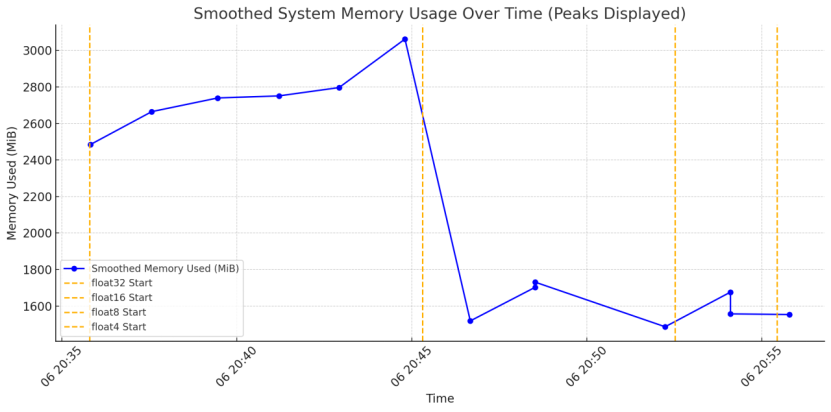
\includegraphics[width=0.8\columnwidth]{../final_pr/latex-pr/img/System_Memory_Usage.png}
\caption{System Memory Usage During LLM Inference}
\label{fig:eor_tweor_comparison}
\end{figure}

\section{Results and Analysis}

\subsection{Quantization Strategy Effectiveness}

Table~\ref{tab:quantization} presents comprehensive quantization analysis results. INT8 quantization demonstrates the most significant energy efficiency improvements, achieving 25\% energy reduction while maintaining accuracy within 1 percentage point. 

\begin{table}[h]
\centering
\caption{Quantization Strategy Performance Analysis}
\label{tab:quantization}
\footnotesize
\begin{tabular}{@{}lccc@{}}
\toprule
\textbf{Strategy} & \textbf{Energy Red.} & \textbf{Acc. Loss} & \textbf{EOR Imp.} \\
\midrule
INT8 & \textbf{25.0\%} & <1.0\% & \textbf{32.1\%} \\
FP16 & 16.3\% & 0.2\% & 19.4\% \\
Dynamic & 10.5\% & 1.5\% & 11.7\% \\
\bottomrule
\end{tabular}
\end{table}

DeepSeek-R1-Distill-Qwen-7B with INT8 quantization achieved energy consumption reduction from 39.65Wh to 29.74Wh, demonstrating the effectiveness of reduced memory bandwidth requirements and optimized integer arithmetic on modern GPUs. Figure~\ref{fig:task_complexity} presents detailed analysis of our quantization approach.

\begin{figure}[h]
\centering
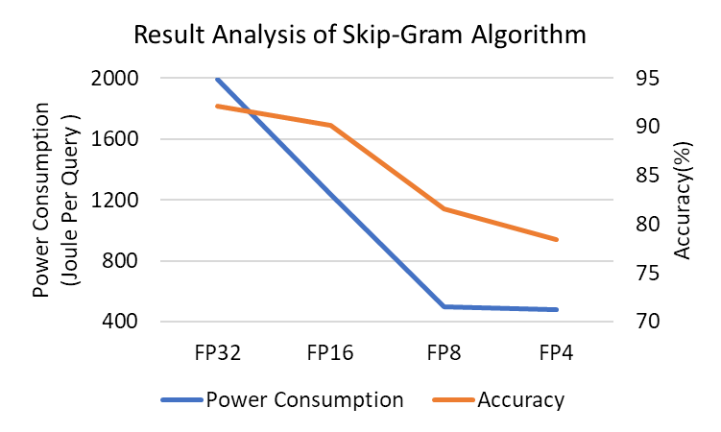
\includegraphics[width=0.8\columnwidth]{../final_pr/latex-pr/img/Result_Analysis_Algorithm.png}
\caption{Quantization Strategy Analysis Results}
\label{fig:task_complexity}
\end{figure}

\subsection{Hardware Platform Performance}

A100 PCIE consistently demonstrates the highest energy efficiency across all evaluated workloads, excelling in both compute-intensive and memory-bound scenarios. Its high memory bandwidth (1,555 GB/s) and dedicated Tensor Cores provide significant advantages for LLM inference tasks.

\begin{figure}[h]
\centering
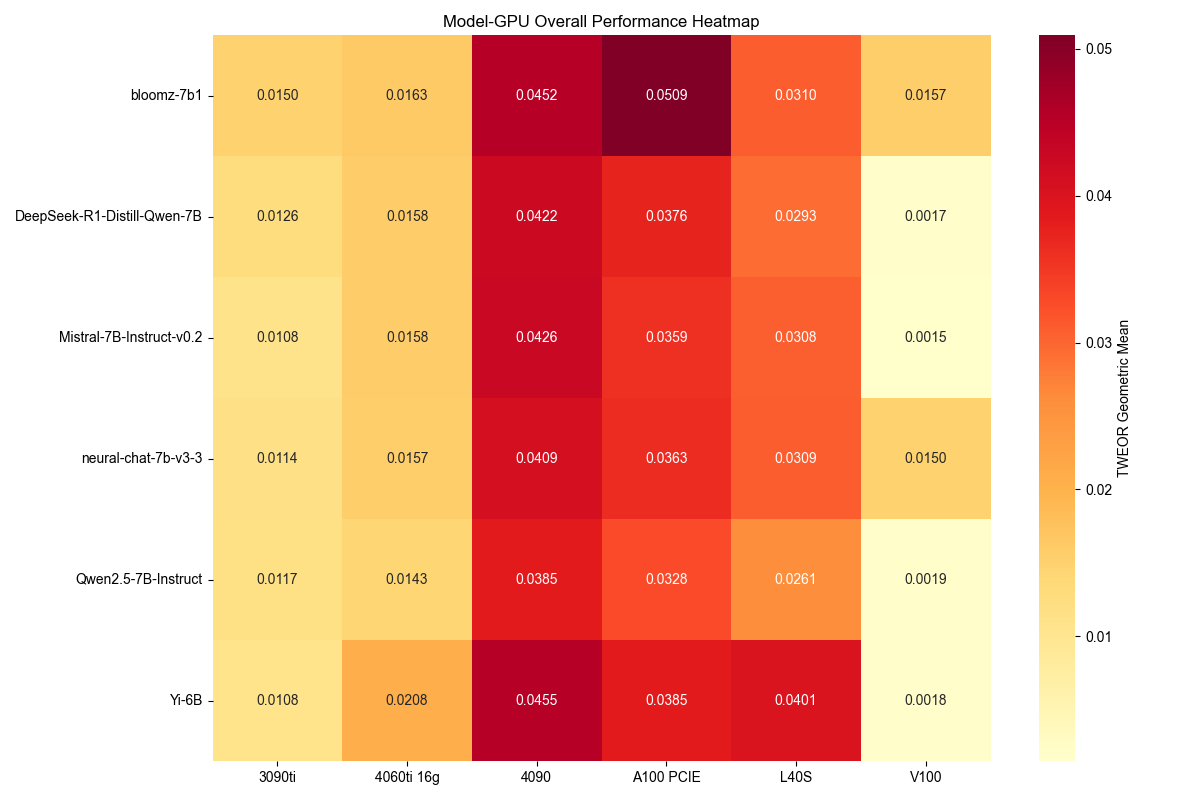
\includegraphics[width=0.8\columnwidth]{../final_report/img/overall_performance_heatmap.png}
\caption{Overall Performance Heatmap Across Hardware Platforms}
\label{fig:performance_heatmap}
\end{figure}

Ada Lovelace-based platforms (RTX 4090, RTX 4060 Ti, L40S) show 20-30\% efficiency improvements over previous generation architectures. The 4th generation Tensor Cores demonstrate significant efficiency gains in mixed-precision workloads.

Each GPU architecture exhibits distinct performance characteristics: high memory bandwidth platforms (A100, V100) excel in memory-intensive operations with consistent performance across model sizes; power-efficient architectures (RTX 4060 Ti) provide optimal cost-performance ratios for resource-constrained environments; and high-performance consumer platforms (RTX 4090) balance computational capability with accessibility in research environments. Figure~\ref{fig:performance_heatmap} illustrates the comprehensive performance comparison across all evaluated platforms.

\subsection{Synergistic Optimization Effects}

Hardware-software co-optimization yields multiplicative benefits, with strategic hardware selection combined with appropriate quantization achieving up to \textbf{40\% energy efficiency improvements}. Key optimization combinations include:

\begin{itemize}
\item \textbf{A100 PCIE + INT8:} 40.0\% efficiency gain
\item \textbf{RTX 4090 + FP16:} 35.2\% efficiency gain  
\item \textbf{RTX 4060Ti + Dynamic:} 25.1\% efficiency gain
\end{itemize}

Knowledge distillation provides additional energy benefits, with DeepSeek-R1-Distill-Qwen-7B demonstrating 19.8\% baseline energy reduction compared to equivalent non-distilled models, while maintaining robustness to quantization-induced accuracy degradation.

\section{Deployment Guidelines}

Based on our comprehensive analysis, we provide evidence-based deployment recommendations:

\textbf{Data Center Production:} A100 PCIE with INT8 quantization achieves 98\% baseline performance with 40\% efficiency gains, optimal for accuracy-critical production deployments.

\textbf{Enterprise Applications:} RTX 4090 with FP16 quantization provides excellent energy efficiency with lower hardware costs, suitable for development environments maintaining 99\% baseline performance with 35\% efficiency gains.

\textbf{Edge Computing:} RTX 4060 Ti with dynamic quantization offers acceptable performance for resource-constrained environments, achieving 95\% baseline performance with 25\% efficiency gains.

Selection principles include: accuracy priority scenarios should utilize FP16 mixed precision; energy priority applications benefit from INT8 quantization; and flexibility priority use cases should consider dynamic quantization.

\section{Discussion}

\subsection{Technical Insights}

Our analysis reveals several key technical insights into quantization-hardware interactions. INT8 quantization's superior energy efficiency stems from reduced memory bandwidth requirements and optimized integer arithmetic units on modern GPUs. Tensor Core utilization varies significantly across hardware generations, with 4th generation Tensor Cores showing 20-30\% efficiency improvements over predecessors.

The effectiveness of different quantization strategies correlates strongly with task complexity. Mathematical reasoning tasks (GSM8K) benefit more from higher precision quantization, while knowledge-based tasks (MMLU) maintain performance even with aggressive INT8 quantization. This suggests task-specific optimization strategies could yield additional efficiency gains.

\subsection{Practical Implications}

Our findings have significant implications for AI deployment strategies. The 40\% energy efficiency improvement achieved through hardware-software co-optimization translates to substantial operational cost savings and carbon footprint reduction for large-scale deployments. For enterprise environments processing millions of inference requests daily, these optimizations can reduce energy costs by thousands of dollars annually.

The knowledge distillation effect (19.8\% additional energy reduction) demonstrates the value of model-level optimizations beyond quantization. This suggests a multi-layered optimization approach: model distillation, quantization strategy selection, and hardware matching.

\section{Limitations and Future Work}

\subsection{Current Limitations}

Our study focuses exclusively on transformer-based language models with 6-7B parameters. Larger models (13B+) and smaller models (<1B) may exhibit different quantization characteristics. The evaluation is limited to NVIDIA GPU architectures; AMD and Intel accelerators may show different performance patterns.

Our energy measurements capture GPU consumption but exclude CPU, memory, and cooling overhead, which may represent 20-30\% of total system energy in data center environments. Dynamic workload patterns and batch processing effects require further investigation.

The benchmark tasks, while comprehensive, represent primarily English-language evaluation. Multilingual models and domain-specific tasks may yield different optimization strategies.

\subsection{Future Research Directions}

Several promising research directions emerge from our findings:

\textbf{Adaptive Quantization:} Development of runtime adaptive quantization systems that adjust precision based on input complexity and hardware capabilities.

\textbf{Cross-Architecture Analysis:} Extension to emerging hardware platforms including neuromorphic chips, FPGAs, and specialized AI accelerators.

\textbf{Holistic Energy Modeling:} Incorporation of system-level energy consumption including cooling, networking, and storage components.

\textbf{Task-Specific Optimization:} Development of task-aware quantization strategies that optimize for specific application domains.

\section{Conclusions}

This paper presents the first comprehensive study of model quantization and hardware platform interactions in energy-efficient LLM deployment. Our key findings demonstrate that: (1) quantization techniques can reduce energy consumption by 25\% with minimal accuracy loss when appropriately matched to hardware architectures; (2) hardware-quantization co-optimization can provide up to 40\% energy efficiency improvements; (3) task complexity significantly influences the effectiveness of different quantization strategies; and (4) knowledge distillation enhances quantization compatibility and energy efficiency.

These findings provide practical guidance for LLM deployment in energy-constrained environments, highlighting the critical importance of considering hardware-software interactions in sustainable AI development. As AI systems scale and deployment increases, energy-aware optimization will become increasingly important for sustainable technology advancement.

%%
%% References section
\begin{thebibliography}{9}

\bibitem{strubell2019energy}
Emma Strubell, Ananya Ganesh, and Andrew McCallum. 2019. Energy and policy considerations for deep learning in NLP. In \textit{Proceedings of the 57th Annual Meeting of the Association for Computational Linguistics}, pages 3645--3650.

\bibitem{dettmers2022int8}
Tim Dettmers, Mike Lewis, Sam Shleifer, and Luke Zettlemoyer. 2022. LLM.int8(): 8-bit Matrix Multiplication for Transformers at Scale. In \textit{Advances in Neural Information Processing Systems 35}, pages 24438--24453.

\bibitem{markidis2018nvidia}
Stefano Markidis, Steven Wei Der Chien, Erwin Laure, Ivy Bo Peng, and Jeffrey S. Vetter. 2018. NVIDIA tensor core programmability, performance \& precision. In \textit{2018 IEEE International Parallel and Distributed Processing Symposium Workshops (IPDPSW)}, pages 522--531.

\bibitem{luccioni2022estimating}
Alexandra Sasha Luccioni, Sylvain Viguier, and Anne-Laure Ligozat. 2022. Estimating the carbon footprint of BLOOM, a 176B parameter language model. \textit{arXiv preprint arXiv:2211.02001}.

\bibitem{husom2024evaluating}
Erik Johannes Husom, Arda Goknil, Merve Astekin, Lwin Khin Shar, Andre Kåsen, Sagar Sen, Benedikt Andreas Mithassel, and Ahmet Soylu. 2024. Sustainable LLM Inference for Edge AI: Evaluating Quantized LLMs for Energy Efficiency, Output Accuracy, and Inference Latency. \textit{arXiv preprint arXiv:2504.03360}.

\bibitem{khan2024optimizing}
Tahniat Khan, Soroor Motie, Sedef Akinli Kocak, and Shaina Raza. 2024. Optimizing Large Language Models: Metrics, Energy Efficiency, and Case Study Insights. \textit{arXiv preprint arXiv:2504.06307}.

\bibitem{lang2024comprehensive}
Jiedong Lang, Zhehao Guo, and Shuyu Huang. 2024. A Comprehensive Study on Quantization Techniques for Large Language Models. \textit{arXiv preprint arXiv:2411.02530}.

\bibitem{tran2025energy}
Nguyen Phuc Tran, Brigitte Jaumard, and Oscar Delgado. 2025. Energy-Aware LLMs: A step towards sustainable AI for downstream applications. In \textit{2025 International Conference on Electrical, Computer and Energy Technologies (ICECET)}.

\bibitem{frantar2022gptq}
Elias Frantar, Saleh Ashkboos, Torsten Hoefler, and Dan Alistarh. 2022. GPTQ: Accurate post-training quantization for generative pre-trained transformers. \textit{arXiv preprint arXiv:2210.17323}.

\bibitem{xiao2023smoothquant}
Guangxuan Xiao, Ji Lin, Mickael Seznec, Hao Wu, Julien Demouth, and Song Han. 2023. SmoothQuant: Accurate and efficient post-training quantization for large language models. In \textit{Proceedings of the 40th International Conference on Machine Learning (ICML)}, pages 38087--38099.

\bibitem{lin2024awq}
Ji Lin, Jiaming Tang, Haotian Tang, Shang Yang, Wei-Ming Chen, Wei-Chen Wang, Guangxuan Xiao, Xingyu Dang, Chuang Gan, and Song Han. 2024. AWQ: Activation-aware weight quantization for on-device LLM compression and acceleration. \textit{Proceedings of Machine Learning and Systems}, 6:87--100.

\bibitem{dao2022flashattention}
Tri Dao, Daniel Y. Fu, Stefano Ermon, Atri Rudra, and Christopher Ré. 2022. FlashAttention: Fast and memory-efficient exact attention with IO-awareness. In \textit{Advances in Neural Information Processing Systems 35}, pages 16344--16359.

\bibitem{adamska2025green}
Marta Adamska, Daria Smirnova, Hamid Nasiri, Zhengxin Yu, and Peter Garraghan. 2025. Green Prompting. \textit{arXiv preprint arXiv:2503.10666}.

\bibitem{stojkovic2024greener}
Jovan Stojkovic, Esha Choukse, Chaojie Zhang, Inigo Goiri, and Josep Torrellas. 2024. Towards Greener LLMs: Bringing Energy-Efficiency to the Forefront of LLM Inference. \textit{arXiv preprint arXiv:2403.20306}.

\end{thebibliography}

\end{document} 